\chapter{Sériová komunikace}
\label{Sériová komunikace}

%Sériová komunikace je posílání dat v řadě nebo-li bit po bitu
Seriová komunikace je způsob přenosu dat mezi dvěma nebo více zařízeními, při kterém se data posílají po jednotlivých bitech po jediném vodiči nebo bezdrátovém kanálu. Seriová komunikace je vhodná pro dlouhé vzdálenosti a nižší rychlosti, protože vyžaduje méně vodičů než paralelní komunikace, která se běžně využívá na deskách plošných spojů. Seriová komunikace se dělí na synchronní a asynchronní, podle toho, zda je potřeba precizně synchronizovat časování při vysílání mezi vysílačem a přijímačem. Pro naše účely se budem zabývat pouze asychronní komunikací. Seriová komunikace se používá pro různé účely, jako je komunikace s modemem, tiskárnou, senzory, paměťovými kartami, síťovými adaptéry a dalšími periferiemi. Běžné a obecně známé standardy a protokoly pro seriovou komunikaci jsou RS-232, UART, SPI, USB.
%...precizně synchronizovat časování při vysílání mezi vysílačem a přijímačem (tohle poradil Pety)
\cite{ser kom}
%[zdroj]
%zdroj kniha o seriove komunikaci
\begin{figure}[!h]
    \begin{center}
        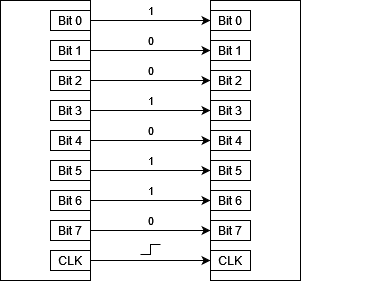
\includegraphics[scale=0.62]{obrazky/paralelni_komunikace.png}
        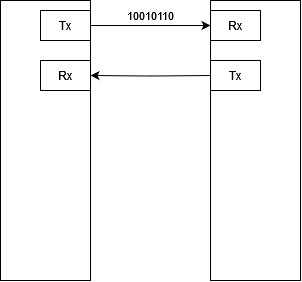
\includegraphics[scale=0.62]{obrazky/Seriova komunikace.png}
    \end{center}
    \caption[Porovnání seriové a paralelní komunikace]{Porovnání paralelní(vlevo) a sériové(vpravo) komunikace. Sériová komunikace v topologii pro UART protokol}
\end{figure}
%zdroj: https://www.rohde-schwarz.com/cz/products/test-and-measurement/essentials-test-equipment/digital-oscilloscopes/understanding-serial-protocols_254522.html#gallery-5

%\section{Komunikační protokoly}
%Komunikační protokol je sada pravidel a dohod, které umožňují zařízením komunikovat mezi sebou. Protokol definuje formát, obsah, časování a řízení toku dat mezi odesílatelem a příjemcem. \cite{ser kom}

\section{UART protokol}
Komunikační protokol je sada pravidel a dohod, které umožňují zařízením komunikovat mezi sebou. Protokol definuje formát, obsah, časování a řízení toku dat mezi odesílatelem a příjemcem.

UART (Universal asynchronous receiver - transmitter) protokol je jeden z nejstarších a nejjednodušších komunikačních protokolů, který používá sériovou linku pro přenos dat mezi dvěma zařízeními. UART protokol nemá společný hodinový signál, ale zařízení se mezi sebou jinými prostředky dohodnou na rychlosti přenosu (baud rate) a formátu dat (počet bitů, parita, stop bit). UART protokol používá čtyři signály: TX (vysílač), RX (přijímač), GND (zem) a volitelně RTS/CTS (řízení toku). \cite{ser kom} %UART protokol je často používán pro komunikaci s periferními zařízeními, jako jsou modemy, senzory, displeje nebo klávesnice. \cite{ser kom}

\subsection{UART datový paket}
\label{UARTt}
Datový paket popisuje posloupnost nebo-li datový tok bitů. Z obrázku č. \ref{UART packet} je vidět, že paket je ohraničený START(logická úrověň 1) a STOP(logická úrověň 0) bitem, které udávají začátek a konec zprávy. Díky tomu jsme schopni separovat více jdoucích paketů v řadě. Za START bitem následuje datový rámec, který býva z pravidla 8 bitový (1 Bajt) a nese informaci uživatele, ostatní bity slouží k "řízení" paketu. Dále je zde paritní bit, který aplikuje na datový rámec logickou operaci XOR. Existují dva druhy parity: sudá - XOR operace je rovna 1 pokud počet jedniček v datovém rámci je sudý.  Pro lichou paritu platí to stejné v případě, že počet jedniček v rámci je lichý. Paritní bity nejsou vždy využity. Záleží na konkrétní aplikaci. Slouží ke kontrole, jestli datový rámec není poškozen. \cite{ser kom} %[zdroj:] %https://cs.wikipedia.org/wiki/Paritn%C3%AD_bit
%*XOR je 

\begin{figure}[!h]
    \begin{center}
        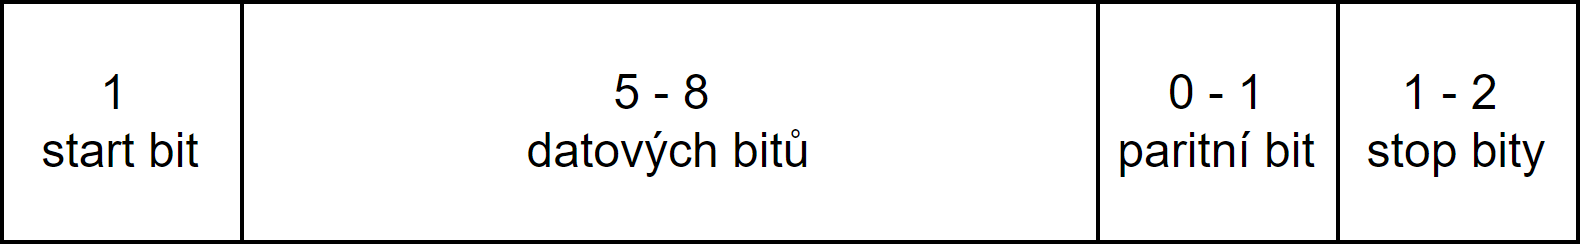
\includegraphics[scale=0.5]{obrazky/datovy ramec UART - final.png}
    \end{center}
    \caption{Datový tok protokolu UART}
    \label{UART packet}
\end{figure}
%ZDROJ: https://yarkov.tech/en/blog/2022-11-04/using-the-web-serial-api-to-communicate-with-the-microcontroller/

\section{Standard RS-232}
Komunikační standard je soubor pravidel a specifikací, které definují, jak mají zařízení komunikovat mezi sebou. Komunikační standard zahrnuje fyzické, elektrické, funkční a mechanické charakteristiky komunikačního rozhraní. Například RS-232 je komunikační standard pro sériovou komunikaci mezi počítačem a modemem.
RS-232 definuje:
\begin{itemize}
    \item \textbf{Elektrické charakteristiky:} RS-232 používá napěťové úrovně od -15 V do +15 V pro reprezentaci logických stavů 0 a 1. RS-232 také specifikuje maximální rychlost přenosu, impedanci, toleranci zkratu a další parametry signálu.
    \item \textbf{Funkční charakteristiky:} RS-232 popisuje funkce a smysl definovaných signálů, které se používají pro řízení toku dat mezi zařízeními. Některé z těchto signálů jsou například: TXD (odesílaná data), RXD (přijímaná data), RTS (požadavek na odeslání), CTS (povolení k odeslání) a DTR (připraven k zařízení).
    \item \textbf{Mechanické charakteristiky:} RS-232 definuje také fyzický tvar a rozmístění pinů konektorů, které se používají pro propojení zařízení. Nejběžnějšími typy konektorů jsou DB9 a DB25, které mají devět a pětadvacet pinů, viz obrázek č.\ref{rs232_obr} \cite{ser kom}
\end{itemize}
%Zdroj dokument o seri. komunikaci

\begin{figure}[!h]
    \begin{center}
        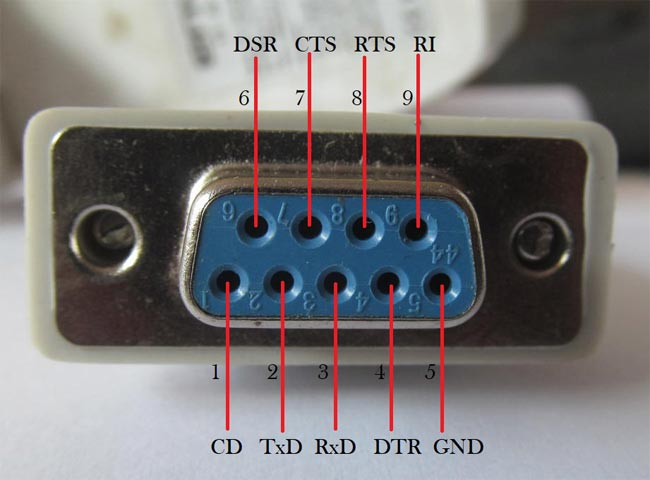
\includegraphics[scale=0.4]{obrazky/RS232.jpeg}
    \end{center}
    \label{rs232_obr}
    \caption{Konektor DB9 s popisem pinů. \cite{RS232}}
\end{figure}
%zdroj RS-232: https://www.pbxdom.com/blog/engineering/what-is-serial-rs232-port-interface/

%\section{USB}
%Universal Serial Bus zkráceně USB je průmyslový standard, který stanovuje specifikace pro kabely a konektory na zařízeních, stéjně jako výše zmíněné RS-232.
%
%USB diponuje konektory Vcc (napájení 5V), datovými piny D+ (vysílač), D- (přijímač) a GND(zem). Obsahuje další konektory jako superrychlostní datové piny, ale těmi se zabívat nebudeme.
%
%Existuje několik verzí USB, které se od sebe líší jak fyzickými rozměry(tvarem konektoru) tak i přenosovou rychlostí. My se budem zabívat verzí USB 2.0 a 3.x s konektorem typu A
%
%USB přišlo jako "náhrada" za starší standard RS-232. USB je rozměrově menší a několika násobně rychlejší.[zdroj]
%%zdroj ai, citoval wikinu
%
%%asi vymazat tuhle sračku
%\begin{figure}[!h]
%    \begin{center}
%        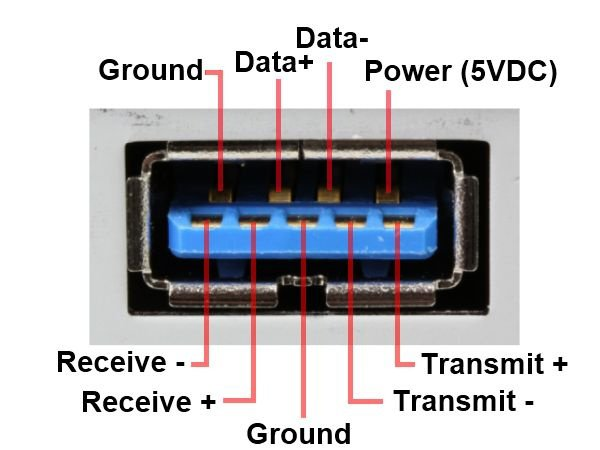
\includegraphics[scale=0.4]{obrazky/USB.jpg}
%    \end{center}
%    \caption{USB 3.1/3.2 A s popisem pinů}
%\end{figure}
%%zdroj USB: https://www.quora.com/If-USB-3-0-type-A-support-max-output-at-5v-0-9a-why-are-there-so-many-type-A-to-type-C-cables-that-supposedly-support-5v-3a
%%Doporuceno zmenit zdroj